\documentclass[11pt]{article}
\usepackage[utf8]{inputenc}
\usepackage[T1]{fontenc}
\usepackage{amsmath,amssymb,amsfonts}
\usepackage{graphicx}
\usepackage{booktabs}
\usepackage{hyperref}
\usepackage{xcolor}
\usepackage[margin=1in]{geometry}
\usepackage[numbers]{natbib}
\usepackage{enumitem}

\newcommand{\oq}{\text{O/Q}}
\newcommand{\dwnorm}{\|\Delta W\|/\|W\|}
\newcommand{\modeldelta}{\textsc{modeldelta}}

\title{The Weight-Space O/Q Ratio: A Robust Fingerprint of LLM \\
Post-Training Regimes and an R1-Distillation Scaling Pattern}

\author{
Nikolay Yudin \\
Independent Researcher \\
\texttt{n.yudin@gmail.com}
}

\date{\today}

\begin{document}
\maketitle

% ======================================================================
% ABSTRACT
% ======================================================================
\begin{abstract}

We introduce the \emph{O/Q ratio}---the ratio of mean relative Frobenius norms
of weight deltas in the output projection ($\mathbf{W}_O$) versus the query
projection ($\mathbf{W}_Q$) of transformer attention layers---as a lightweight,
architecture-portable metric for characterizing post-training regimes of large
language models.
Computing O/Q requires only the base and fine-tuned checkpoints: no forward
passes, no training data, and no GPU.
Across 59 model pairs (52 fully profiled, 7 O/Q-only) spanning 10
architecture families (with an O/QKV variant for fused-projection
architectures), we show that weight-only O/Q cleanly separates R1-style
knowledge distillation ($\oq > 2$) from all other post-training types,
which cluster near $\oq \approx 1$.
Most notably, O/Q for DeepSeek-R1 distilled models follows a log-linear
trend with parameter count across five lineage-matched sizes from 1.5\,B to 32\,B
($\oq = 1.04 \ln B + 1.13$, $R^2{=}0.82$, $p{=}0.035$), with a supportive
70\,B point on an approximate base confirming the trend.
Standard post-training O/Q remains flat ($0.82$--$0.96$) across the same size
range.
Targeted negative controls show that neither chain-of-thought training data,
reinforcement learning, nor model scale alone produce elevated O/Q, consistent
with an effect specific to R1's distillation recipe.
All analysis code is released as the open-source \modeldelta{} toolkit
(\url{https://github.com/nick-yudin/modeldelta}).

\end{abstract}


% ======================================================================
% 1. INTRODUCTION
% ======================================================================
\section{Introduction}

The rapid proliferation of fine-tuned language model checkpoints on platforms
such as HuggingFace has created a fundamental transparency problem.
As of early 2026, thousands of model variants are publicly available, yet
the training recipes behind them---supervised fine-tuning (SFT), reinforcement
learning from human feedback (RLHF), direct preference optimization (DPO),
knowledge distillation, domain specialization, or combinations thereof---are
frequently undocumented, partially documented, or described only at a high
level.
This opacity makes it difficult for practitioners to select models, predict
compatibility for merging, or audit provenance.

A natural question arises: \emph{can we characterize what kind of post-training
a checkpoint underwent by examining its weights alone?}
In this work, we answer affirmatively for a specific but informative signal.
We show that the relative magnitude of weight changes in different attention
projection types---specifically, the output projection versus the query
projection---carries a surprisingly robust signature of the training recipe.

We define the \textbf{O/Q ratio} as the ratio of mean relative Frobenius norms
of weight deltas in the output projection ($\mathbf{W}_O$) over the query
projection ($\mathbf{W}_Q$) across all transformer layers.
This scalar metric is:
\begin{itemize}[nosep]
  \item \textbf{Architecture-portable}: O/Q values for matched training types
    are consistent across transformer families with separate O and Q projections,
    and extend to fused-QKV architectures via an O/QKV variant.
  \item \textbf{Lightweight}: it requires only two checkpoints and can be
    computed on CPU in minutes, even for 70\,B-parameter models via selective
    shard downloading.
  \item \textbf{Discriminative}: O/Q separates six categories of post-training
    with minimal overlap.
\end{itemize}

Our central finding is a \emph{scaling pattern unique to R1-distillation}.
Among all 59 model pairs analyzed, only DeepSeek-R1 distilled models exhibit
O/Q that grows log-linearly with parameter count---from $\sim$2.0 at 1.5\,B to
$\sim$5.3 at 32\,B across five lineage-matched points, with a supportive 70\,B
point ($\oq \approx 7.9$) on an approximate base confirming the trend.
A matched control experiment using Qwen3 standard post-training (SFT~+~RL)
across five model sizes shows flat O/Q ($0.82$--$0.96$), confirming that the
scaling pattern is not a general effect of model size or training intensity.

\paragraph{Contributions.}
\begin{enumerate}[nosep]
  \item We propose the weight-only O/Q ratio and demonstrate its portability
    across 10 transformer families (with an O/QKV variant for fused-projection
    architectures).
  \item We show that O/Q $> 2$ reliably identifies R1-distillation across
    59 model pairs, while all other post-training types cluster near $\oq \approx 1$.
  \item We discover a log-linear O/Q scaling pattern specific to R1-distillation
    ($R^2{=}0.82$, five lineage-matched points, with a supportive sixth point)
    and confirm its absence in standard post-training.
  \item We provide targeted negative controls showing that chain-of-thought data,
    RL, and model scale alone do not produce elevated O/Q in our experiments.
  \item We release \modeldelta{}, a pip-installable CLI tool that computes all
    reported metrics from any HuggingFace checkpoint pair.
\end{enumerate}


% ======================================================================
% 2. RELATED WORK
% ======================================================================
\section{Related Work}

\paragraph{Weight-space analysis and model merging.}
Low-rank structure in weight updates has been studied extensively since
LoRA~\citep{hu2022lora} demonstrated that fine-tuning changes occupy a low-rank
subspace.
\citet{matena2022fisher} introduced Fisher-weighted averaging, showing that
parameter importance varies across layers and tensor types---a key early result
that not all weight changes are equally informative.
\citet{choshen2022fusing} demonstrated that simply averaging fine-tuned model
weights produces better base models for downstream tasks, and
\citet{donyehiya2023cold} extended this to collaborative multitask fusing.
These results established that the \emph{distribution} of weight changes across
model components carries meaningful signal.
Model soups~\citep{wortsman2022model} showed that averaging multiple fine-tuned
checkpoints improves accuracy without additional compute.
Task arithmetic~\citep{task-arithmetic} formalized the idea of adding and
subtracting task-specific weight deltas, and
TIES-Merging~\citep{yadav2023ties} addressed interference when combining
such deltas.
Subsequent work unified these perspectives:
\citet{jin2023regmean} formulated merging as minimizing prediction discrepancy
using activation statistics, while \citet{daheim2024gradient} showed that
Fisher merging and task arithmetic both implicitly project into task-specific
subspaces.
\citet{yang2024merging-survey} provide a comprehensive survey of model merging
methods and applications.
More recently, \citet{merging-collapse} showed that parameter-space metrics
fail to predict whether merged models retain capabilities, arguing that
representation-level divergence is the true predictor---a finding our own
experiments confirm (Section~\ref{sec:discussion}).
Our work differs from all of the above in that we do not merge or manipulate
weight deltas, but rather analyze their per-projection-type structure as a
\emph{diagnostic fingerprint} of how training was conducted.

\paragraph{Post-training methods.}
The standard post-training pipeline involves SFT followed by
RLHF~\citep{ouyang2022training} or DPO~\citep{rafailov2023dpo}.
More recently, DeepSeek-R1~\citep{deepseek-r1} introduced a distillation
approach where reasoning capabilities are transferred from a large RL-trained
model to smaller models via fine-tuning on curated reasoning traces.
Several concurrent efforts pursue reasoning via RL
(Phi-4-reasoning~\citep{phi4}, QwQ, EXAONE-Deep) or SFT on long chain-of-thought
traces (s1, OpenThinker~\citep{openthinker}).
Our O/Q metric distinguishes these approaches in weight space.

\paragraph{Scaling laws.}
Scaling laws relating model performance to compute, data, and parameters are
well established~\citep{kaplan2020scaling, chinchilla}.
Recent work has also examined scaling of test-time compute~\citep{jain2024neftune}.
To our knowledge, we present the first empirical scaling trend in
\emph{weight-delta space}: a systematic relationship between model size and the
structure of training-induced weight changes.


% ======================================================================
% 3. METHOD
% ======================================================================
\section{Method}

\subsection{Weight Delta Computation}

Given a base model $\theta_\text{base}$ and a fine-tuned model $\theta_\text{ft}$
with matching architecture, we compute per-tensor relative Frobenius norms:
\begin{equation}
  \text{relative norm}(i) = \frac{\|\theta_\text{ft}^{(i)} - \theta_\text{base}^{(i)}\|_F}{\|\theta_\text{base}^{(i)}\|_F}
  \label{eq:relnorm}
\end{equation}
where $i$ indexes individual weight tensors.
This normalization makes the metric comparable across layers and model sizes,
as it measures \emph{proportional} change rather than absolute magnitude.

Our implementation streams safetensor shards sequentially, requiring only enough
memory to hold one tensor at a time.
For 70\,B-parameter models where only O/Q is needed, we selectively download
only the shards containing attention projection weights (reducing the download
from $\sim$141\,GB to $\sim$25\,GB).
Figure~\ref{fig:pipeline} illustrates the full pipeline.

\begin{figure}[t]
  \centering
  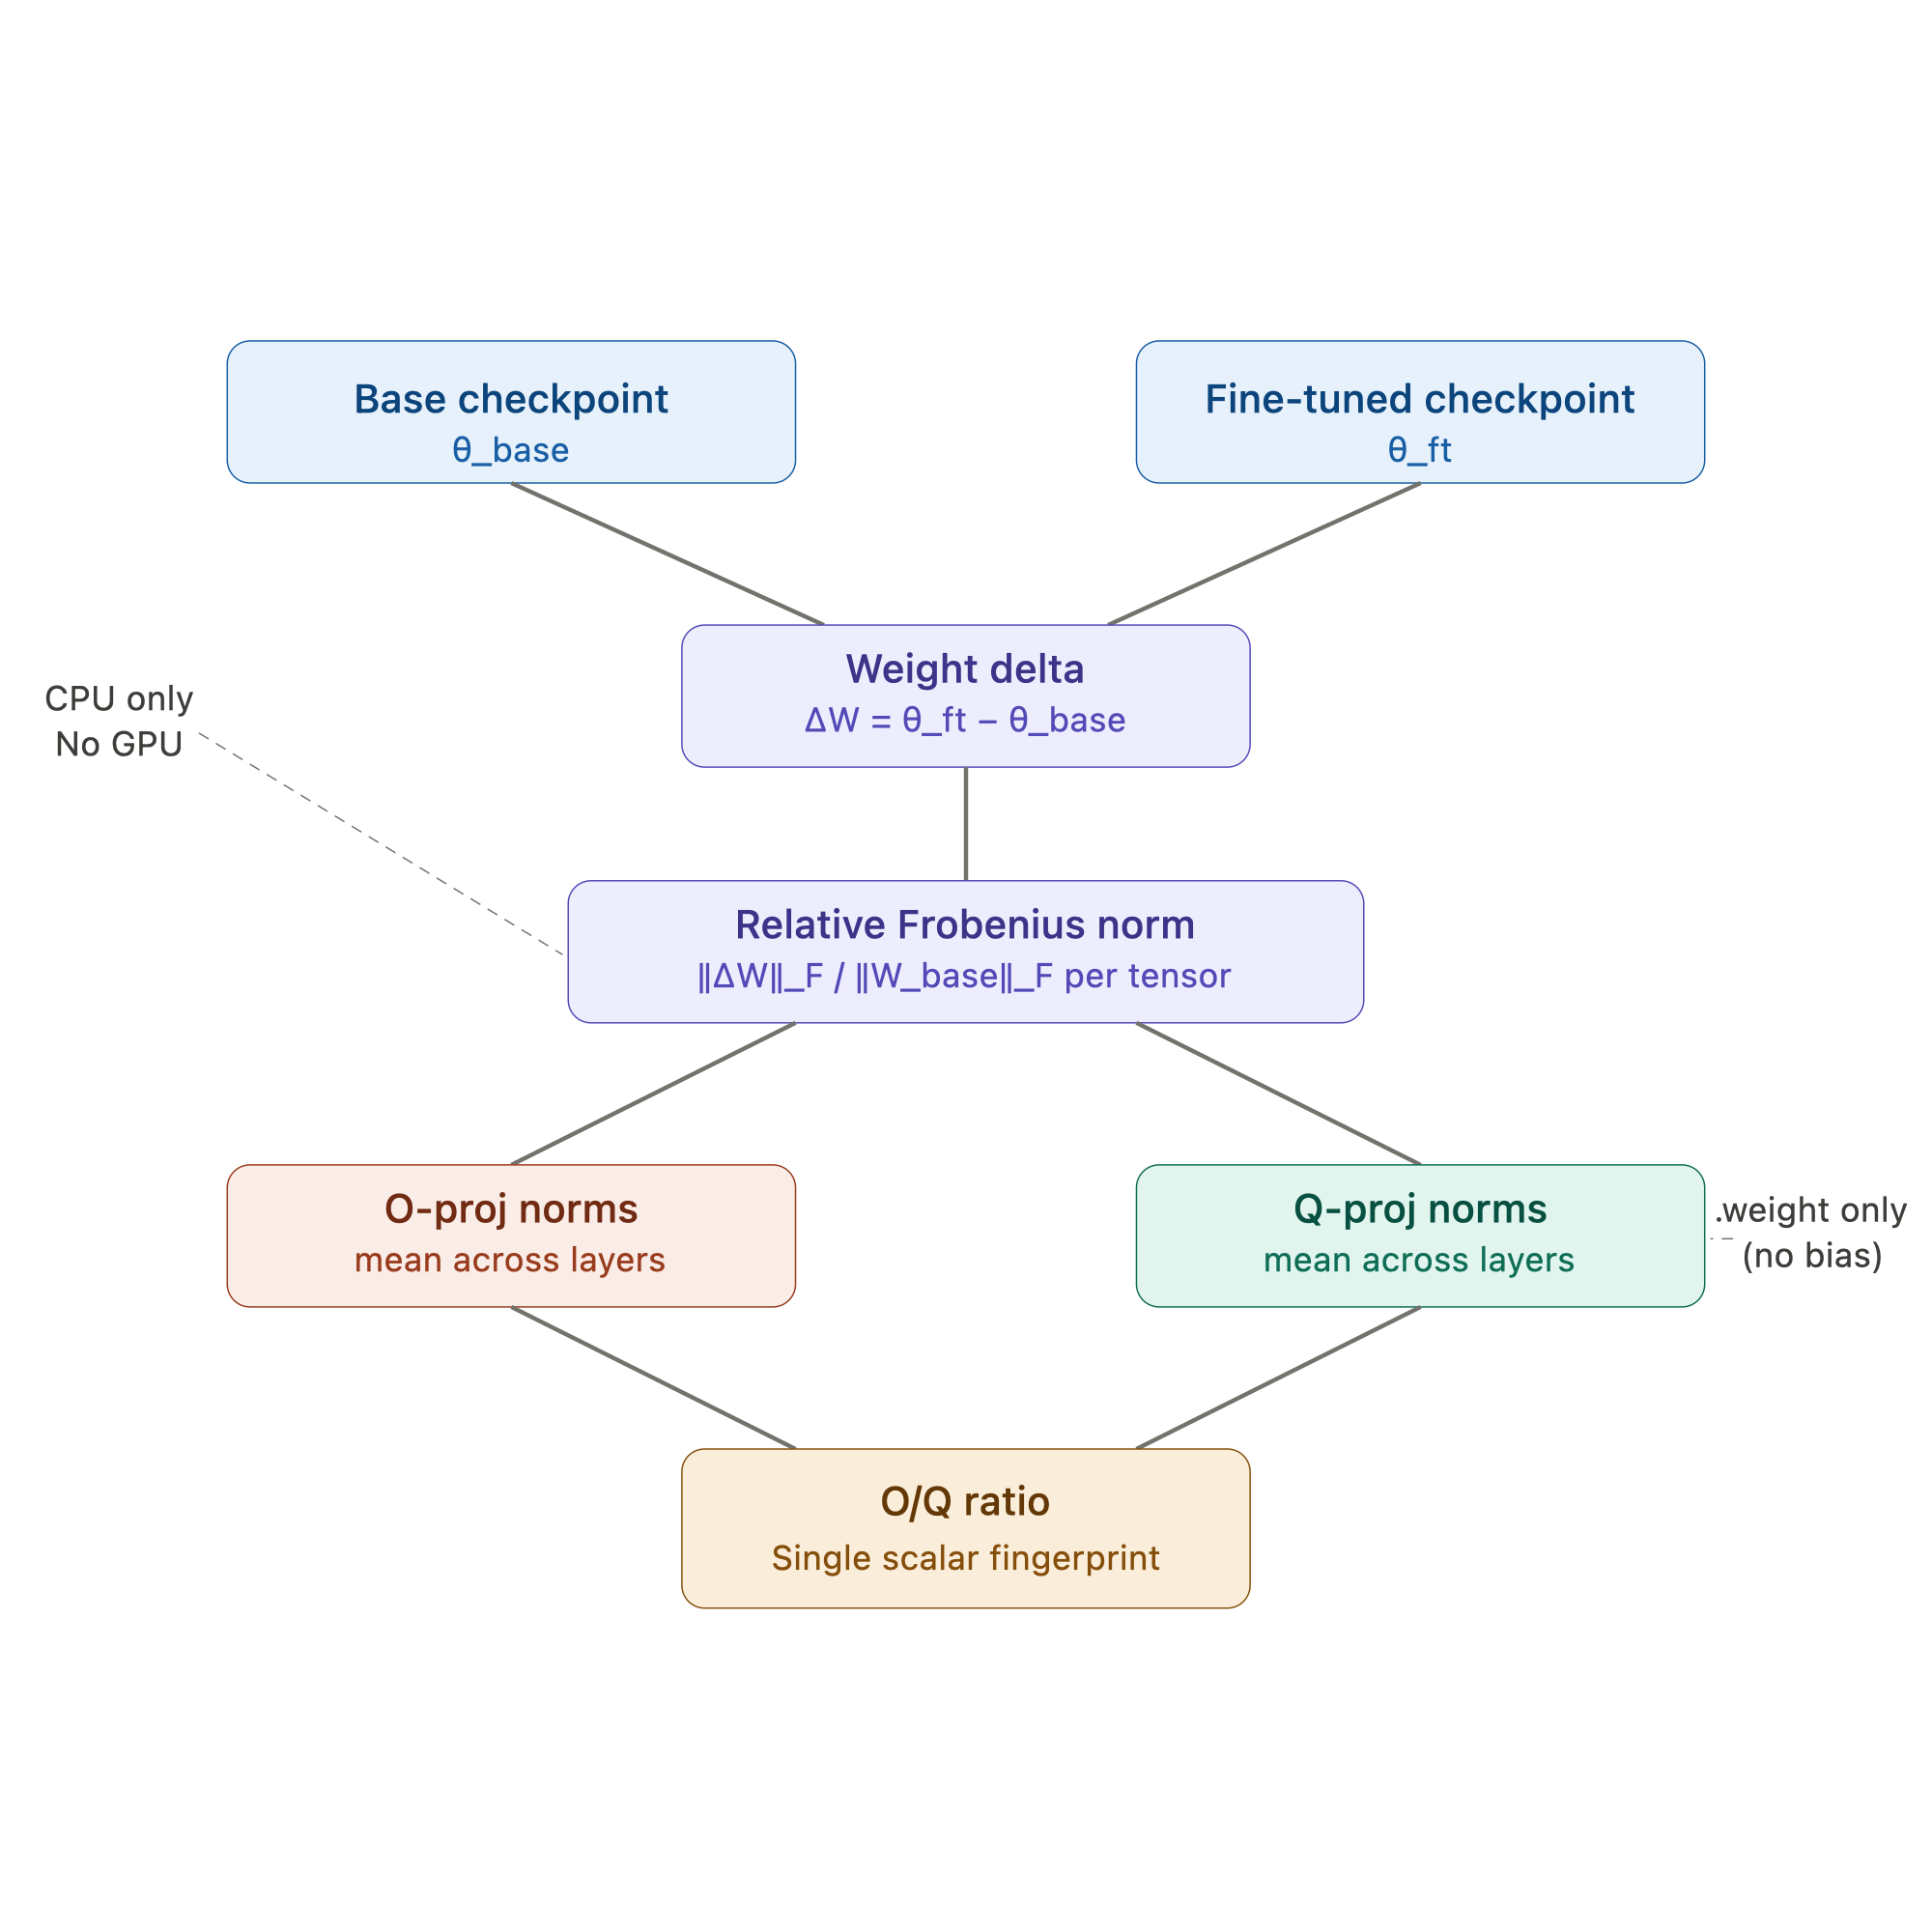
\includegraphics[width=0.65\textwidth]{figures/oq_method_pipeline.png}
  \caption{O/Q computation pipeline.
    Two checkpoints are differenced tensor-by-tensor, relative Frobenius norms
    are computed, then grouped by projection type and averaged across layers to
    produce a single scalar.
    The entire process runs on CPU with no forward passes.}
  \label{fig:pipeline}
\end{figure}

\subsection{The O/Q Ratio}
\label{sec:oq-def}

We define the O/Q ratio as:
\begin{equation}
  \oq = \frac{\text{mean}_{l} \; \text{relative norm}_{l}^{(\text{o\_proj.weight})}}{\text{mean}_{l} \; \text{relative norm}_{l}^{(\text{q\_proj.weight})}}
  \label{eq:oq}
\end{equation}
where $l$ indexes transformer layers, and the numerator and denominator average
the relative Frobenius norms of output projection weights and query projection
weights, respectively.

\paragraph{Weight-only computation.}
We restrict O/Q computation to \texttt{.weight} tensors only, excluding bias
terms.
This is methodologically important: some architectures (e.g., Qwen) include
\texttt{q\_proj.bias} but no \texttt{o\_proj.bias}.
Including bias terms in the averaging introduces a systematic asymmetry that
inflates O/Q in affected families (see Appendix~\ref{app:bias}).
The weight-only definition ensures cross-architecture comparability.

\paragraph{Architecture alias mapping.}
Different transformer families use different naming conventions for attention
projections.
We map architecture-specific names to canonical O and Q categories:
\begin{itemize}[nosep]
  \item \textbf{Standard} (Qwen, Llama, Mistral, Gemma, OLMo, Yi):
    \texttt{o\_proj} / \texttt{q\_proj}
  \item \textbf{EXAONE}: \texttt{out\_proj} / \texttt{q\_proj}
  \item \textbf{Phi}: fused \texttt{qkv\_proj}; O/Q becomes O/QKV
  \item \textbf{Falcon, InternLM}: fused \texttt{query\_key\_value} or
    \texttt{wqkv}; O/Q becomes O/QKV
\end{itemize}
For architectures with fused QKV projections, we compute O/QKV rather than O/Q.
Since the fused QKV tensor combines query, key, and value weights, the
denominator is not identical to a standalone Q projection; O/QKV values fall in
a similar range but should be interpreted as a related variant rather than an
exact equivalent.

\paragraph{Intuition.}
The output projection $\mathbf{W}_O$ controls how attention heads combine
information (output mixing), while the query projection $\mathbf{W}_Q$ controls
what heads attend to (query formation).
O/Q measures the balance of training signal between these two functions
(Figure~\ref{fig:attn}).
An O/Q $\gg 1$ indicates that training disproportionately modified the output
mixing circuitry, while O/Q $\approx 1$ indicates balanced modification.

\begin{figure}[t]
  \centering
  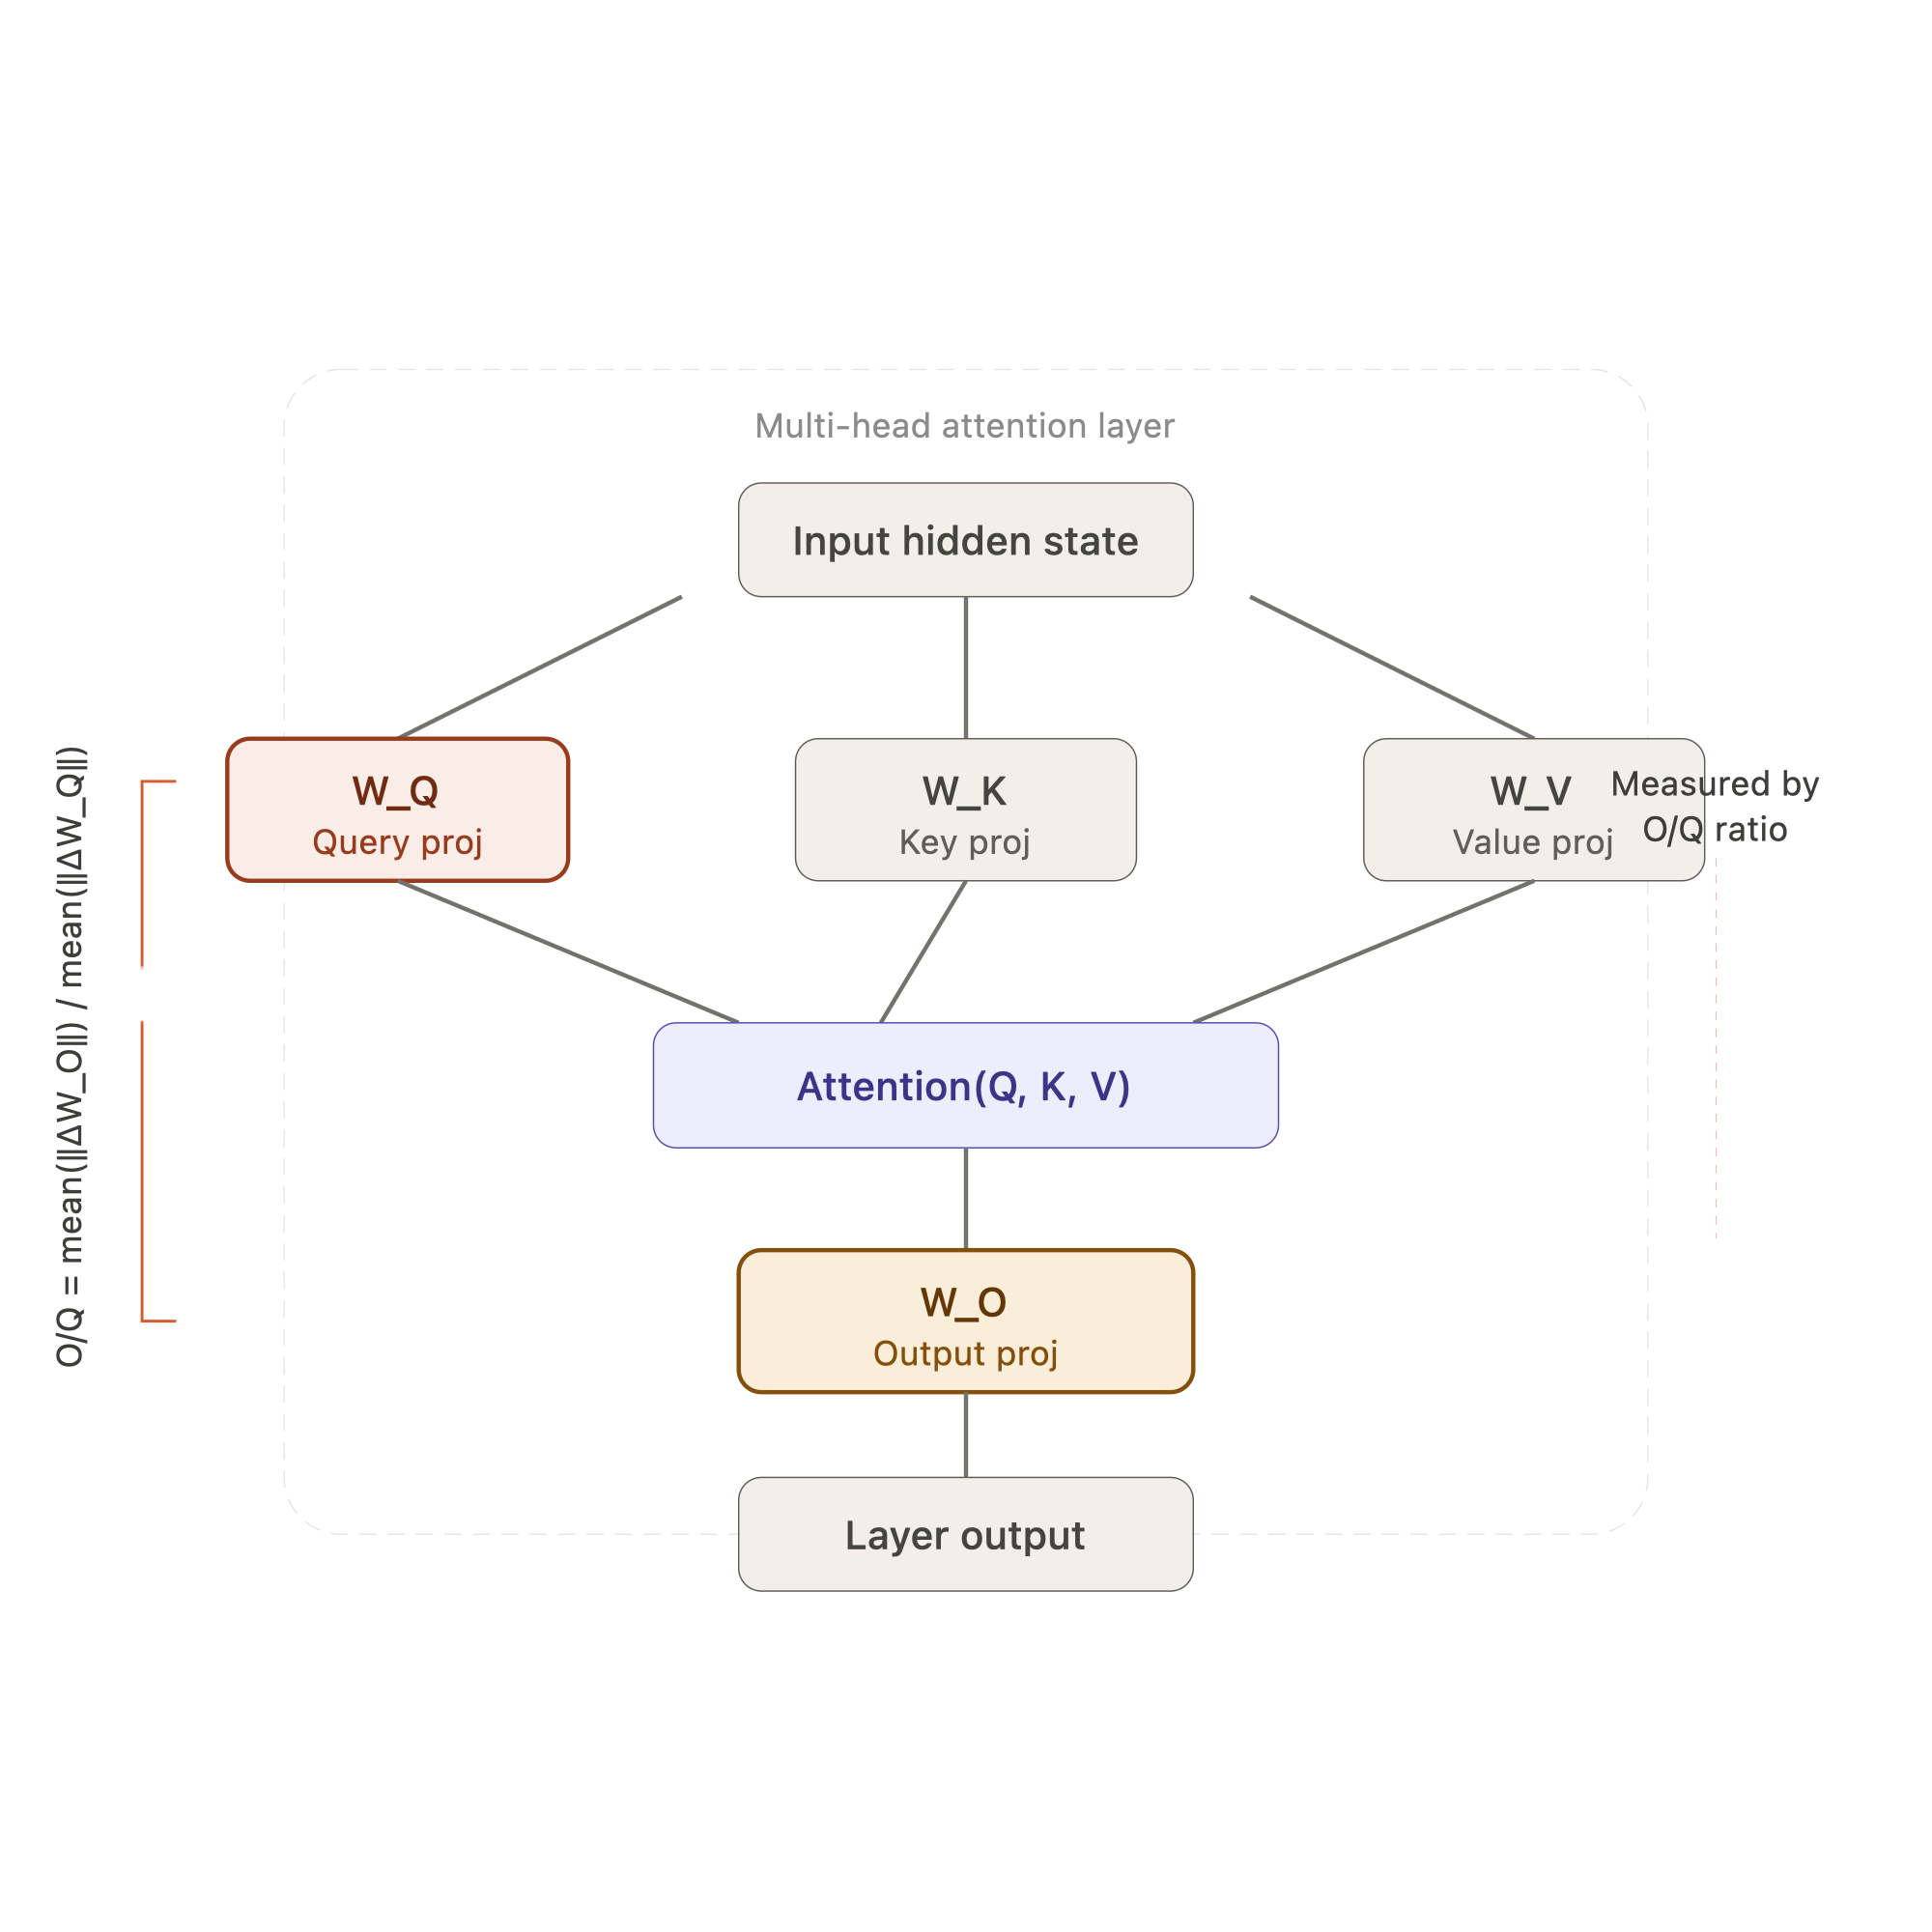
\includegraphics[width=0.55\textwidth]{figures/attention_block_oq_highlight.png}
  \caption{Attention block with the two projections compared by O/Q
    highlighted: $\mathbf{W}_Q$ (query formation) and $\mathbf{W}_O$
    (output mixing). $\mathbf{W}_K$ and $\mathbf{W}_V$ are not used in the
    ratio.}
  \label{fig:attn}
\end{figure}


\subsection{Additional Metrics}

Beyond O/Q, \modeldelta{} computes several complementary metrics for each
model pair:
\begin{itemize}[nosep]
  \item \textbf{Global $\dwnorm$}: mean relative Frobenius norm across all
    tensors, measuring overall training magnitude.
  \item \textbf{Cosine similarity}: $\cos(\theta_\text{base}^{(i)},
    \theta_\text{ft}^{(i)})$, measuring directional preservation.
  \item \textbf{Top-$k$ concentration}: fraction of squared singular values of
    $\Delta W$ captured by the top $k$ singular values, measuring low-rank
    structure in the delta.
  \item \textbf{Budget vectors}: 8-dimensional vectors encoding the relative
    magnitude of weight changes across attention projection types
    (Q, K, V, O, gate, up, down, norm).
\end{itemize}


% ======================================================================
% 4. EXPERIMENTAL SETUP
% ======================================================================
\section{Experimental Setup}

\subsection{Model Pairs}

We analyze 59 model pairs spanning 10 architecture families:
Qwen~\citep{qwen25, qwen3}, Llama~\citep{llama3}, Mistral (including Mixtral),
Gemma, Phi~\citep{phi4}, OLMo, EXAONE, Falcon, InternLM, and Yi.
Of these, 45 are fully profiled and categorized by training type,
7 are fully profiled but used only in specific analyses (version evolution,
controls), and 7 are O/Q-only comparisons for large models (70\,B) or scaling
controls (Qwen3 series).

We categorize pairs into six primary training types based on publicly available
documentation:
\begin{enumerate}[nosep]
  \item \textbf{R1-distill}: fine-tuned on DeepSeek-R1 reasoning traces~\citep{deepseek-r1}
  \item \textbf{Community SFT}: community-trained models without DPO (Dolphin, OpenHermes)
  \item \textbf{Standard instruct}: official SFT~+~DPO/RLHF pipelines
  \item \textbf{Non-R1 reasoning}: RL-based or CoT-SFT reasoning (Phi-4-reasoning,
    QwQ, EXAONE-Deep, s1, OpenThinker)
  \item \textbf{Domain specialization}: continued training for math or code
  \item \textbf{Base$\to$SFT}: supervised fine-tuning only (OLMo stage chain)
\end{enumerate}

Additionally, we analyze DPO incremental steps (SFT$\to$DPO), version evolution
pairs, and the Qwen3 post-training control series.

\subsection{R1-Distill Base Model Selection}

The DeepSeek-R1 distilled models use different base models at different scales:
Qwen2.5-Math-1.5B and -7B for the smallest sizes, general Qwen2.5 for 14B and
32B, and Llama-3.1-8B for the 8B variant~\citep{deepseek-r1}.
For 70B, the official base is Llama-3.3-70B-Instruct; we use Llama-3.1-70B as
the closest publicly available general base (same architecture, different
training vintage).
Despite this variation in base models, the O/Q scaling pattern is remarkably
consistent across all six points.

\subsection{Lightweight O/Q for Large Models}

For 70\,B-parameter models, full checkpoint comparison would require downloading
$\sim$282\,GB (two models $\times$ $\sim$141\,GB each).
We implement selective shard downloading: by parsing the
\mbox{\texttt{model.safetensors.index.json}} weight map, we identify and download only
the shards containing \texttt{o\_proj} and \texttt{q\_proj} tensors, reducing
the total download to $\sim$25\,GB per model.
O/Q is then computed on CPU using streaming Frobenius norm accumulation.


% ======================================================================
% 5. RESULTS
% ======================================================================
\section{Results}

\subsection{O/Q Is Architecture-Portable}
\label{sec:invariance}

A useful cross-family metric must produce comparable values for the same type
of training regardless of architecture.
For families with separate O and Q projections (Qwen, Llama, Mistral, Gemma,
OLMo, Yi, EXAONE), O/Q is directly comparable.
For families with fused QKV projections (Phi, Falcon, InternLM), we compute
an O/QKV variant using the combined QKV norm as denominator; this produces
values in the same range but is not formally identical.

Table~\ref{tab:taxonomy} shows that standard instruct models span
O/Q $= 0.73$--$1.49$ across families, with the variation primarily reflecting
training recipe intensity (e.g., Llama-3.1-8B-Instruct at 1.49 vs.\
Gemma-2-9b-it at 0.73).

In contrast, top-$k$ singular value concentration---another natural
candidate---varies 7$\times$ by architecture
(Qwen $\approx 0.14$--$0.22$, Gemma $\approx 0.05$--$0.07$, InternLM $\approx 0.03$),
making it unsuitable for cross-family comparison without normalization.

\subsection{Training Type Taxonomy}
\label{sec:taxonomy}

\begin{table}[t]
\centering
\caption{O/Q ratio by post-training type (weight-only computation).
$n$ = number of model pairs.
10 additional pairs (version evolution, Qwen3 scaling controls, Nemotron control)
are used in specific analyses but not categorized here.}
\label{tab:taxonomy}
\begin{tabular}{lcccc}
\toprule
Training type & O/Q range & $\mu$ & $n$ & Families \\
\midrule
R1-distill & 1.99--7.89 & 4.08 & 6 & Qwen, Llama \\
Non-R1 post-training & 0.73--2.12 & 1.04 & 43 & 10 \\
\quad Standard instruct & 0.73--1.49 & 0.99 & 19 & 10 \\
\quad Non-R1 reasoning & 0.87--1.25 & 1.02 & 6 & Qwen, Phi, EXAONE \\
\quad Community SFT & 1.24--2.12 & 1.72 & 6 & Mistral, Llama \\
\quad Domain specialization & 0.89--1.19 & 0.99 & 5 & Qwen, Llama \\
\quad Base $\to$ SFT only & 0.81 & 0.81 & 2 & OLMo \\
\quad DPO step & 0.84--1.85 & 1.10 & 5 & OLMo, Llama \\
\bottomrule
\end{tabular}
\end{table}

Table~\ref{tab:taxonomy} presents O/Q grouped by training type.
The dominant pattern is a clean two-way split.

\textbf{R1-distill is clearly separated from everything else.}
Even the smallest R1-distill O/Q (1.99 at 1.5\,B) exceeds all non-R1 values
except three Mistral-7B community SFT models (1.81--2.12), and the largest
(7.89 at 70\,B) is $8\times$ the non-R1 mean.
The O/Q $> 2$ threshold has zero false positives among 53 non-R1 pairs.

\textbf{Non-R1 post-training clusters near O/Q $\approx 1$.}
Standard instruct ($\mu = 0.99$), non-R1 reasoning ($\mu = 1.02$), domain
specialization ($\mu = 0.99$), and base-to-SFT ($\mu = 0.81$) all occupy the
range 0.73--1.49 with heavy overlap.
O/Q does not distinguish RL-based reasoning from standard instruction tuning---a
practical limitation (see Section~\ref{sec:discussion}).

\textbf{Community SFT is family-dependent, not a universal category.}
Three Mistral-7B models show elevated O/Q (1.81--2.12), but three Llama-2
community SFT models (Vicuna-7B, Vicuna-13B, Nous-Hermes) show 1.24--1.70,
overlapping with standard instruct.
This suggests the elevated O/Q in Mistral community SFT may reflect
architecture- or recipe-specific effects rather than a general property of
community fine-tuning.

Figure~\ref{fig:taxonomy} visualizes the category ranges on a single O/Q axis,
making the overlap between community SFT and the lower end of R1-distill
visible.

\begin{figure}[t]
  \centering
  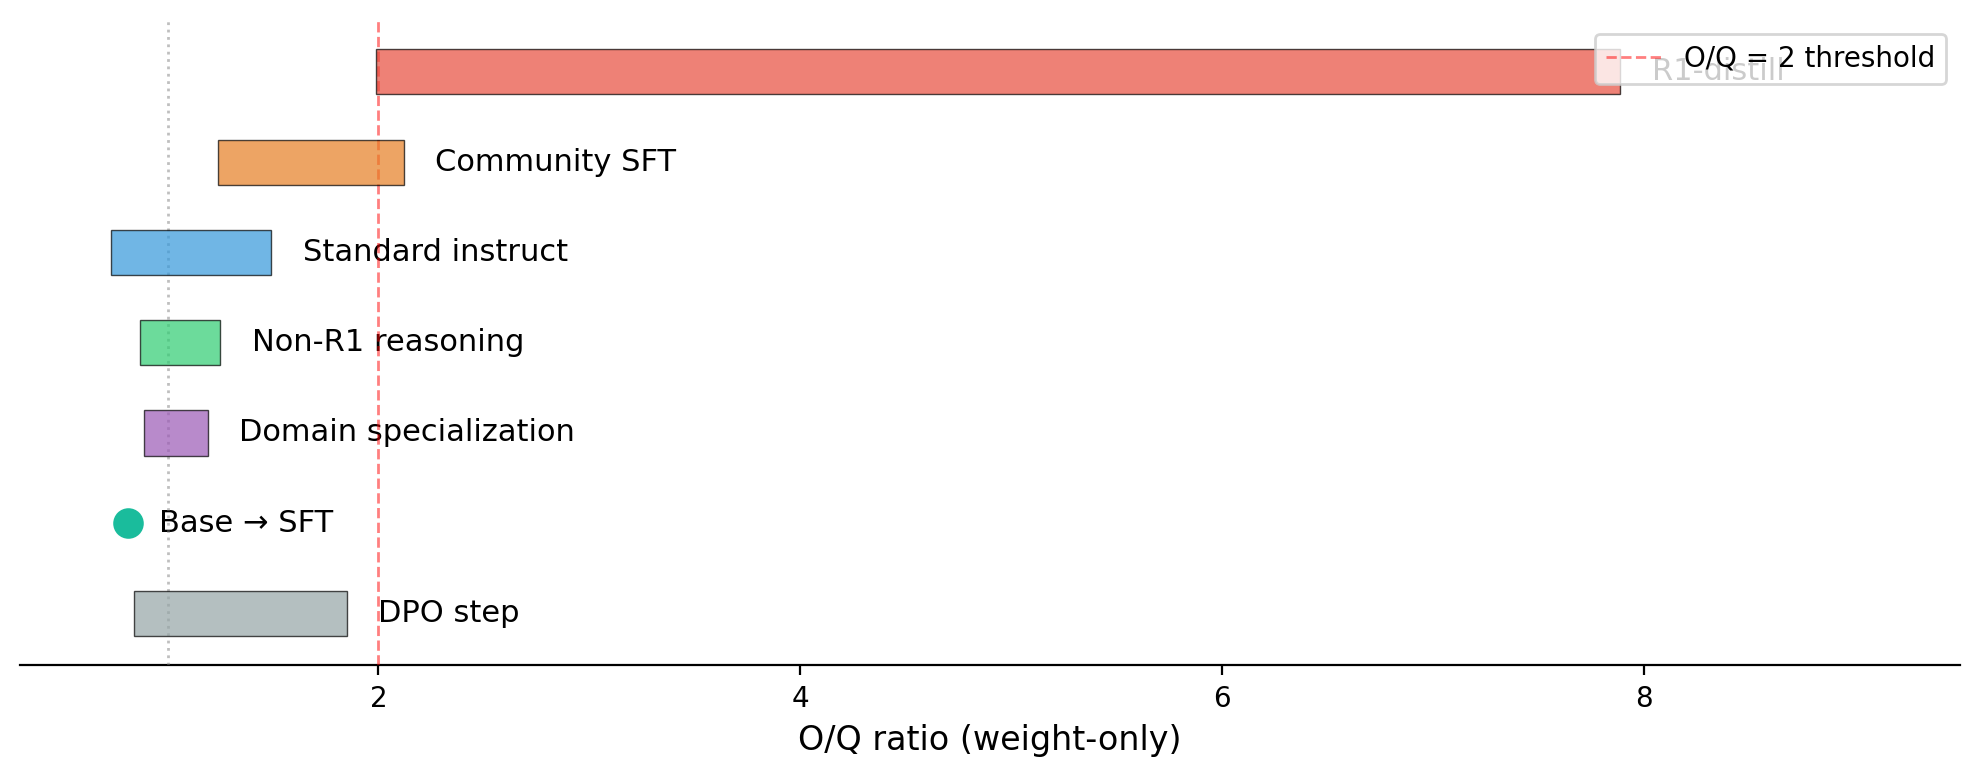
\includegraphics[width=0.85\textwidth]{figures/oq_taxonomy_ranges.png}
  \caption{O/Q ranges for seven post-training categories.
    R1-distillation ($\oq = 1.99$--$7.89$) is cleanly separated above the
    $\oq = 2$ threshold (dashed red line).
    All other categories cluster below 2, with heavy overlap near $\oq \approx 1$.
    Community SFT spans a wide range (1.24--2.12) reflecting family-dependent
    variation (Mistral vs.\ Llama).}
  \label{fig:taxonomy}
\end{figure}

\subsection{Statistical Validation}
\label{sec:stats}

To verify that observed O/Q values reflect genuine structure in weight deltas
rather than sampling artifacts, we conduct two statistical analyses.

\paragraph{Permutation null distribution.}
For each model pair with full per-tensor data, we randomly permute which
relative norms are assigned to the O-projection vs.\ Q-projection groups
(10,000 permutations), computing O/Q under each permutation.
The resulting null distribution has mean $\approx 1.0$ and standard deviation
$\approx 0.15$--$0.20$ (depending on model architecture), reflecting the
expected O/Q if training changed all projection types uniformly.

All five R1-distill pairs with full data achieve $p < 0.001$: their observed
O/Q values are never produced by random assignment of per-tensor norms.
Given the null standard deviation of $\approx 0.15$--$0.20$, an O/Q of 2.0
represents ${>}5\sigma$ from the null mean of 1.0, making chance occurrence
negligible.
In contrast, most standard instruct and reasoning pairs show $p > 0.05$,
meaning their O/Q $\approx 1$ is consistent with the null---exactly as expected
for balanced training.
Figure~\ref{fig:null} shows representative null distributions for an R1-distill
pair and a standard instruct pair.

\paragraph{Bootstrap confidence intervals.}
We compute 95\% bootstrap CIs by resampling layers (with replacement, 10,000
iterations) and recomputing O/Q for each sample.
CIs are tight for models with 32+ layers (typical width 0.06--0.30) and
do not overlap between R1-distill and non-R1 pairs: the lowest R1-distill CI
is $[1.88, 2.11]$ (1.5\,B), while the highest non-R1 CI is $[1.40, 1.60]$
(Llama-3.1-8B-Instruct).
This confirms that the R1/non-R1 separation is robust and not an artifact of
layer-level variance.

\begin{figure}[t]
  \centering
  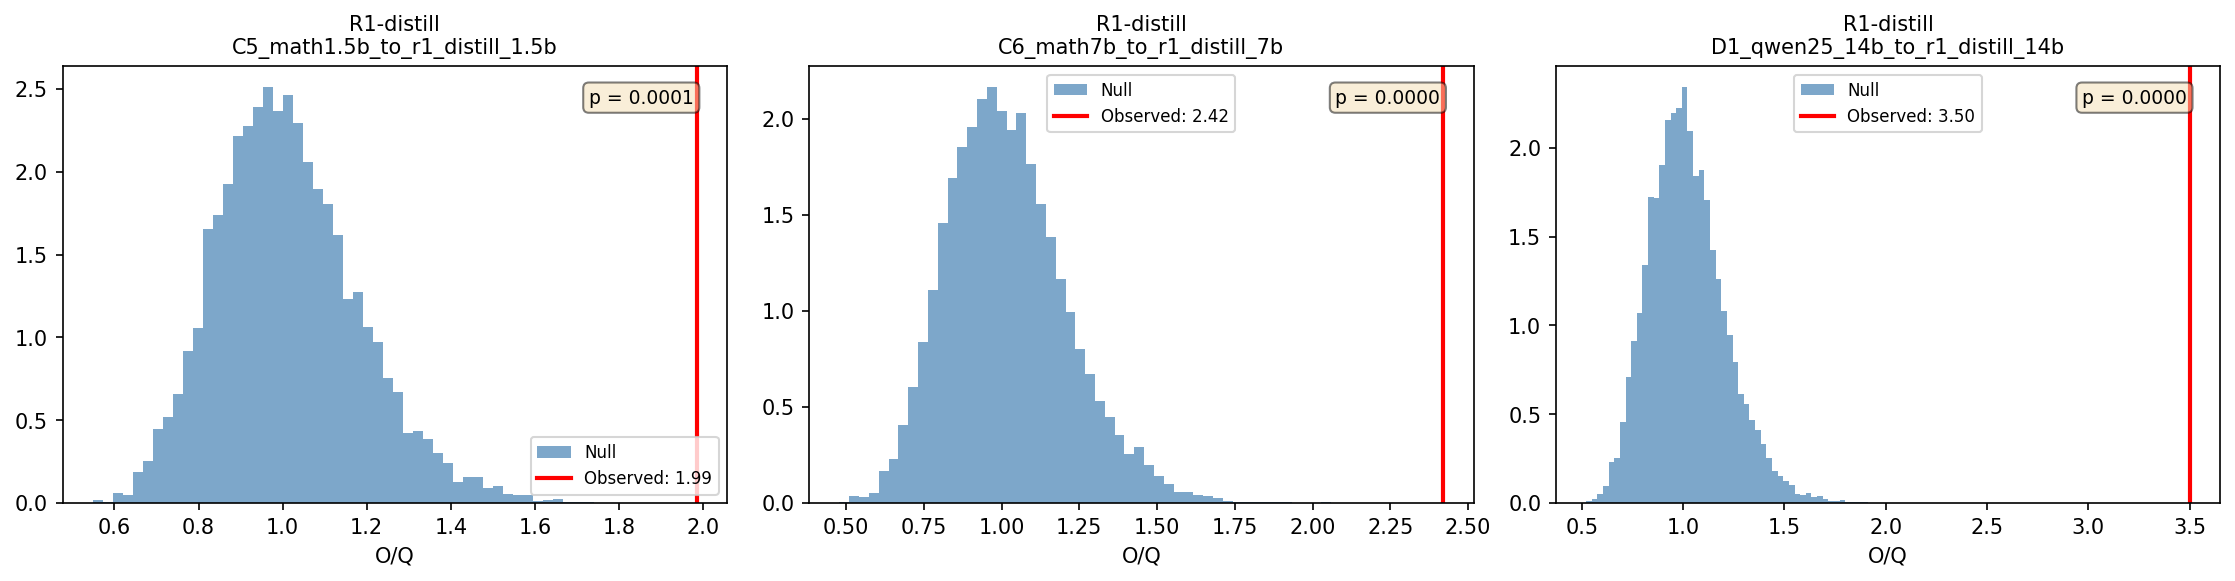
\includegraphics[width=0.85\textwidth]{figures/null_distribution_examples.png}
  \caption{Permutation null distributions (10,000 permutations) for three
    R1-distill pairs at increasing scale: 1.5\,B ($p = 0.0001$), 7\,B
    ($p < 0.0001$), 14\,B ($p < 0.0001$).
    Red lines show observed O/Q; blue histograms show the null.
    Observed values fall far outside the null distribution
    (null mean $\approx 1.0$, SD $\approx 0.17$--$0.19$),
    confirming that the O/Q elevation is not a sampling artifact.}
  \label{fig:null}
\end{figure}


\paragraph{Per-layer profile.}
Figure~\ref{fig:perlayer} shows per-layer relative norms for O-proj and Q-proj
across three representative models.
For R1-distill (32B, left), O-proj norms are uniformly elevated above Q-proj
across all 64 layers---the effect is not concentrated in early or late layers.
For community SFT (OpenHermes, middle), O-proj is above Q-proj but with
substantially more scatter.
For standard instruct (Qwen2.5-7B, right), the two projection types are
nearly interleaved, producing O/Q $\approx 1$.
This uniform elevation across layers for R1-distill suggests a global
architectural effect rather than a localized intervention.
The tight bootstrap CIs at all R1-distill scales (width 0.22--0.34, see
Section~\ref{sec:stats}) are consistent with uniform per-layer elevation
at 1.5\,B and 7\,B as well: if the effect were concentrated in a few layers,
resampling variance would produce wider intervals.

\begin{figure}[t]
  \centering
  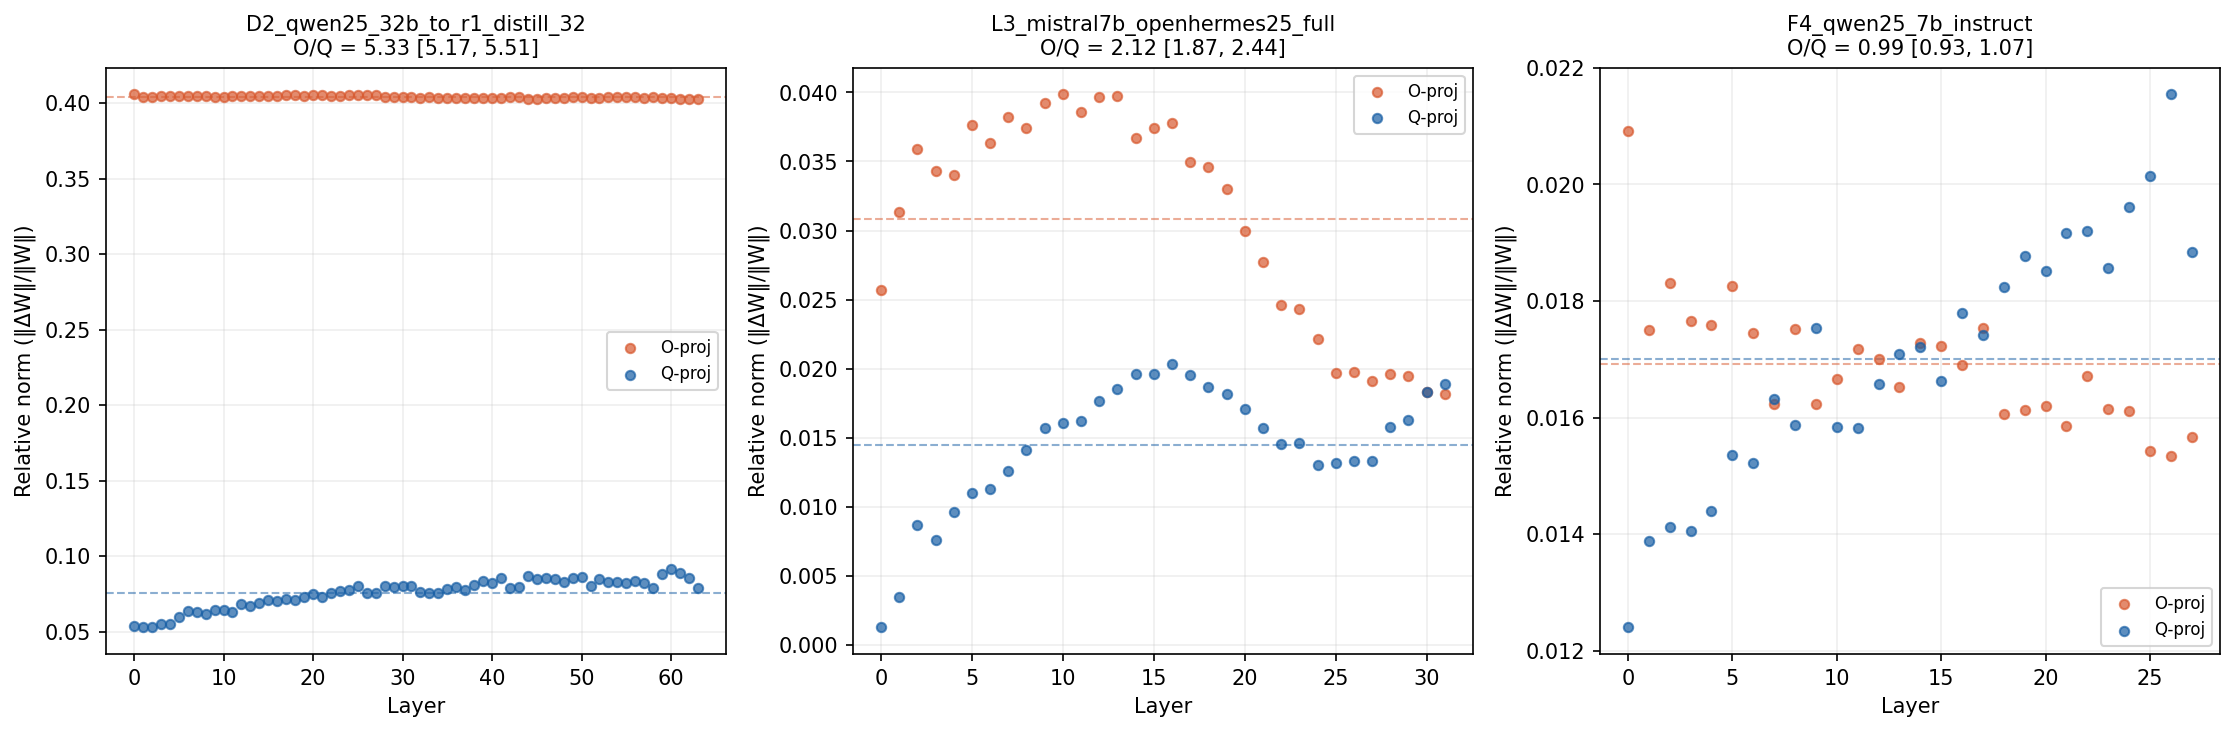
\includegraphics[width=0.95\textwidth]{figures/per_layer_scatter.png}
  \caption{Per-layer relative norms of O-proj (orange) and Q-proj (blue) for
    three models.
    Left: R1-distill 32B ($\oq = 5.33$, O-proj uniformly above Q-proj).
    Middle: community SFT ($\oq = 2.12$, elevated with scatter).
    Right: standard instruct ($\oq = 0.99$, interleaved).
    Dashed lines show per-type means; brackets in titles show 95\% bootstrap
    CIs.}
  \label{fig:perlayer}
\end{figure}


\subsection{R1-Distill O/Q Scaling Trend}
\label{sec:scaling}

\begin{table}[t]
\centering
\caption{R1-distill O/Q by model size.
$\dwnorm$ is the global mean relative Frobenius norm.
$^\dagger$Approximate base: official base is Llama-3.3-70B-Instruct;
we use Llama-3.1-70B (same architecture).}
\label{tab:scaling}
\begin{tabular}{rllcc}
\toprule
Size & Base model & Family & O/Q & $\dwnorm$ \\
\midrule
1.5B & Qwen2.5-Math-1.5B & Qwen & 1.985 & 0.141 \\
7B & Qwen2.5-Math-7B & Qwen & 2.420 & 0.133 \\
8B & Llama-3.1-8B & Llama & 3.343 & 0.150 \\
14B & Qwen2.5-14B & Qwen & 3.501 & 0.093 \\
32B & Qwen2.5-32B & Qwen & 5.334 & 0.072 \\
70B$^\dagger$ & Llama-3.1-70B & Llama & 7.894 & --- \\
\bottomrule
\end{tabular}
\end{table}

Table~\ref{tab:scaling} shows that R1-distill O/Q grows monotonically with
parameter count.
On the five lineage-matched points (1.5\,B--32\,B), a log-linear fit yields:
\begin{equation}
  \oq = 1.04 \cdot \ln(B) + 1.13, \quad R^2 = 0.82, \; p = 0.035
  \label{eq:scaling}
\end{equation}
where $B$ is the parameter count in billions.
Including the 70\,B supportive point (which uses Llama-3.1-70B as an approximate
base; the official R1-distill base is Llama-3.3-70B-Instruct) steepens the
slope ($\oq = 1.51 \ln B + 0.35$, $R^2 = 0.84$, $p = 0.01$), suggesting
the trend continues at larger scales.

Two striking features of this scaling pattern are worth noting:

\textbf{O/Q rises while $\dwnorm$ falls.}
As model size increases, the overall magnitude of weight changes
\emph{decreases} (from 0.141 at 1.5\,B to 0.072 at 32\,B), but these changes
become increasingly concentrated in the output projection.
R1-distillation at larger scales is simultaneously more ``surgical'' (lower
global $\dwnorm$) and more ``focused'' (higher O/Q).

\textbf{Two architecture families follow the trend.}
Both Qwen-based (1.5B, 7B, 14B, 32B) and Llama-based (8B, and the approximate
70\,B point) R1-distill models are consistent with the same curve.

\begin{figure}[t]
  \centering
  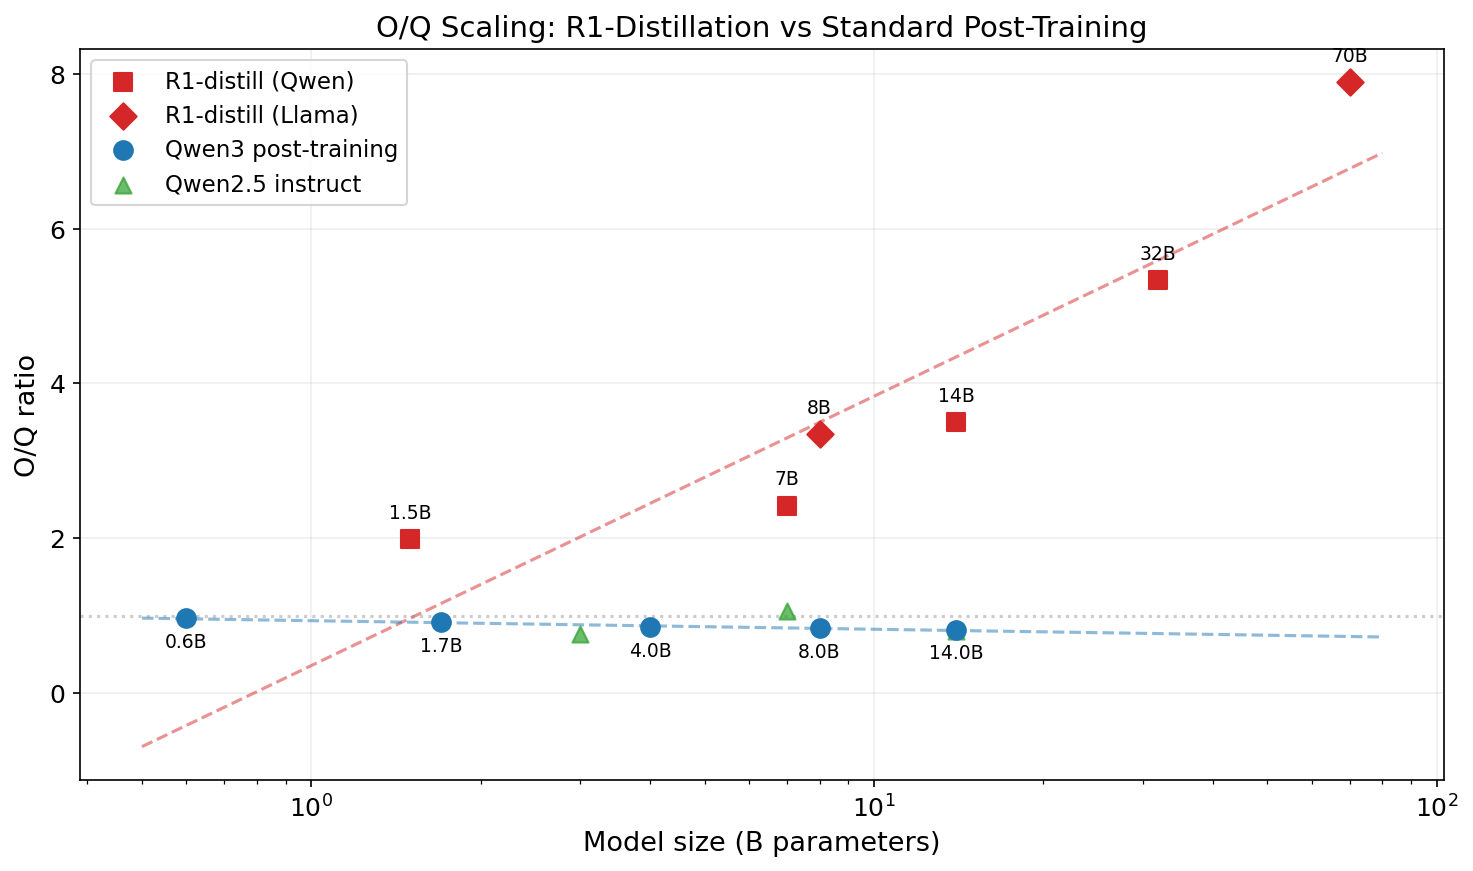
\includegraphics[width=0.85\textwidth]{figures/oq_scaling_r1_vs_qwen3_control.png}
  \caption{O/Q scaling: R1-distill vs.\ Qwen3 standard post-training control.
    R1-distill O/Q grows log-linearly with model size
    ($R^2 = 0.82$ on five lineage-matched points, dashed: six-point fit
    including approximate 70\,B base), while standard post-training
    remains flat.}
  \label{fig:scaling}
\end{figure}


\subsection{Control: Standard Post-Training Is Flat}
\label{sec:control}

To test whether O/Q growth is a general effect of model scale or training
intensity, we constructed a control experiment using Qwen3 models.
The Qwen3 series provides base and post-trained (SFT~+~RL) checkpoints at five
sizes, using standard post-training without R1-distillation~\citep{qwen3}.

\begin{table}[h]
\centering
\caption{Qwen3 Base $\to$ Post-trained O/Q (standard SFT+RL, no R1
distillation).
O/Q is essentially flat across model sizes.}
\label{tab:qwen3}
\begin{tabular}{rc}
\toprule
Size & O/Q \\
\midrule
0.6B & 0.963 \\
1.7B & 0.912 \\
4B & 0.846 \\
8B & 0.834 \\
14B & 0.817 \\
\bottomrule
\end{tabular}
\end{table}

Table~\ref{tab:qwen3} shows that standard post-training O/Q has a slight
negative slope ($-0.05$ on $\ln B$) but remains within the narrow range
$0.82$--$0.96$.
Figure~\ref{fig:scaling} overlays both curves: R1-distill O/Q diverges sharply
from the flat control, with no overlap above 1.5\,B parameters.

An additional 70\,B control confirms this separation at the largest scale:
Nemotron-70B-Instruct (RL-based reasoning, same Llama-3.1-70B base family)
has O/Q $= 1.48$, far below the R1-distill value of 7.89 at the same scale.


\subsection{Negative Controls: What Does Not Cause High O/Q}
\label{sec:negatives}

To narrow down what might drive R1-distill's elevated O/Q, we tested three
alternative hypotheses using observational controls.

\paragraph{Hypothesis 1: Chain-of-thought training data causes high O/Q.}
If the long reasoning traces in R1's training data were the cause, then any
model fine-tuned on similar CoT data should show elevated O/Q.
Two direct tests falsify this:
\begin{itemize}[nosep]
  \item s1-32B (SFT on 1,000 QwQ/o1-mini reasoning traces): O/Q $= 0.905$
  \item OpenThinker-7B (SFT on QwQ reasoning traces): O/Q $= 0.918$
\end{itemize}
Both values fall squarely in the standard instruct/reasoning range.
Long CoT training data alone does not elevate O/Q.

\paragraph{Hypothesis 2: Reinforcement learning causes high O/Q.}
If RL-based reasoning training were the cause, non-R1 RL models should show
similar scaling:
\begin{itemize}[nosep]
  \item Phi-4-reasoning (RL): O/Q $= 1.075$
  \item QwQ-32B (RL): O/Q $= 0.870$
  \item EXAONE-Deep-7.8B (RL): O/Q $= 1.252$
  \item Nemotron-70B (RL): O/Q $= 1.480$
\end{itemize}
All are within or near the standard instruct range.
RL-based reasoning training does not produce the O/Q $> 2$ values characteristic
of R1-distillation.

\paragraph{Hypothesis 3: Model scale alone causes high O/Q.}
The Qwen3 control experiment (Section~\ref{sec:control}) provides evidence
against this: O/Q is flat across model sizes for standard post-training.
The Nemotron-70B control further shows that the 70\,B scale point is not
inherently associated with high O/Q.


\subsection{DPO Contributes an Order of Magnitude Less Change Than SFT}
\label{sec:dpo}

The OLMo-2 model family~provides a rare opportunity to decompose
post-training into individual steps, as checkpoints are released after each
stage (base $\to$ SFT $\to$ DPO $\to$ Instruct).

\begin{table}[h]
\centering
\caption{Training step magnitudes for OLMo-2 models.
DPO and subsequent alignment steps are an order of magnitude smaller than SFT.}
\label{tab:dpo}
\begin{tabular}{llcc}
\toprule
Step & Size & $\dwnorm$ & O/Q \\
\midrule
Base $\to$ SFT & 7B & 0.049 & 0.812 \\
SFT $\to$ DPO & 7B & 0.001 & 0.980 \\
DPO $\to$ Instruct & 7B & 0.0004 & 0.917 \\
\midrule
Base $\to$ SFT & 13B & 0.018 & 0.809 \\
SFT $\to$ DPO & 13B & 0.001 & 0.911 \\
DPO $\to$ Instruct & 13B & 0.001 & 0.841 \\
\bottomrule
\end{tabular}
\end{table}

Table~\ref{tab:dpo} shows a clear hierarchy: SFT produces $\dwnorm \approx
0.02$--$0.05$, while DPO and subsequent alignment contribute $\dwnorm \approx
0.001$ or less---a 20--50$\times$ reduction.
DPO is a fine correction, not a rewrite.
All O/Q values for these incremental steps cluster near 1.0, indicating
balanced modification.

\paragraph{Edge case.}
One DPO step (Tulu-3 SFT$\to$DPO on Llama-3.1-8B) shows O/Q $= 1.85$ despite
$\dwnorm = 0.001$.
We attribute this to ratio instability at very small delta magnitudes: when both
numerator and denominator of Equation~\ref{eq:oq} are near zero, small absolute
differences produce large O/Q values.
This suggests that O/Q is most informative for training steps with
$\dwnorm > 0.01$.


\subsection{Domain Specialization: Large Changes, Balanced Projections}

Domain-specialized models (Math, Coder) exhibit a distinctive profile:
very large weight changes ($\dwnorm = 0.78$--$1.35$) but O/Q $\approx 0.89$--$1.19$,
indicating that these near-complete rewrites distribute changes relatively evenly
across projection types.
This pattern holds across both Qwen (Math, Coder) and Llama (CodeLlama) families.
Domain specialization is the opposite of R1-distillation, which produces moderate
$\dwnorm$ ($0.07$--$0.15$) concentrated in the output projection.

\begin{table}[h]
\centering
\caption{Domain specialization: large overall changes with balanced O/Q.}
\label{tab:domain}
\begin{tabular}{llcc}
\toprule
Pair & Family & $\dwnorm$ & O/Q \\
\midrule
Qwen2.5-7B $\to$ Math-7B & Qwen & 0.951 & 0.923 \\
Qwen2.5-7B $\to$ Coder-7B & Qwen & 0.862 & 0.890 \\
Qwen2.5-14B $\to$ Coder-14B & Qwen & 0.784 & 0.941 \\
Llama-2-7B $\to$ CodeLlama-7B & Llama & 0.966 & 1.190 \\
Llama-2-13B $\to$ CodeLlama-13B & Llama & 1.347 & 1.120 \\
\bottomrule
\end{tabular}
\end{table}




% ======================================================================
% 6. DISCUSSION
% ======================================================================
\section{Discussion}
\label{sec:discussion}

\paragraph{What O/Q reveals about R1-distillation.}
The scaling trend in Equation~\ref{eq:scaling} shows that as model capacity
increases, R1-distillation concentrates its modifications increasingly in the
output projection.
We do not know the mechanistic cause of this pattern.
Without access to R1's training recipe and without interventional experiments
(e.g., freezing specific projection types during distillation), causal
explanation remains out of reach.
What we can say is that the O/Q scaling trend is \emph{empirically unique}:
no other training type among 59 pairs produces it, and the three most natural
alternative explanations (CoT data, RL, model scale) are not supported by our
observational controls.

\paragraph{Confound: heterogeneous base models.}
A key caveat for the scaling trend is that the R1-distill series uses different
base models at different scales (Qwen2.5-Math for 1.5B/7B, general Qwen2.5 for
14B/32B, Llama for 8B/70B).
An alternative hypothesis is that O/Q growth partially reflects differences
between base models rather than a pure scaling property of distillation.
The direction of this potential bias is unclear: the Math-specialized bases at
1.5B/7B are already optimized for mathematical reasoning, which could either
reduce the O-projection delta (if Math-training already shifted O-proj) leading
to \emph{underestimated} O/Q at small scales, or have no systematic directional
effect if Math-specialization distributes changes evenly (as our domain
specialization data suggests: O/Q $\approx 0.92$ for Math).
We note that the Llama-8B point ($\oq = 3.34$) falls on the Qwen-fitted curve
without systematic offset, which would be unlikely under a pure base-model
confound.
However, this does not fully rule out the alternative, and validation on a
single base-model family across sizes---should such R1-distilled models become
available---would substantially strengthen the claim.

\paragraph{Practical applications.}
O/Q has immediate practical utility for model auditing.
Given an unknown fine-tuned model and its base, computing O/Q takes minutes on
CPU and produces a value that can be compared against our taxonomy
(Table~\ref{tab:taxonomy}) to narrow down the likely training recipe.
As a heuristic (not a classifier), O/Q $> 2$ is consistent with R1-distillation
or community SFT without DPO; O/Q $\approx 1$ with standard instruct or
RL-based reasoning; O/Q $< 0.8$ combined with high $\dwnorm$ with domain
specialization.

\paragraph{Limitations.}
Several limitations should be noted:
\begin{enumerate}[nosep]
  \item The primary O/Q scaling fit uses five lineage-matched points.
    While the fit is statistically significant ($p = 0.035$) and absent in
    controls, additional R1-distill sizes would strengthen confidence.
    The 70\,B point uses an approximate base and serves as supportive evidence.
  \item O/Q is \emph{descriptive}, not causal.
    It identifies what happened to a model's weights but cannot explain why a
    specific training recipe produces a specific O/Q pattern.
  \item Our dataset is skewed toward Qwen-family models (27 of 59 total entries).
    While we verify key findings across other families, broader coverage would
    strengthen universality claims.
  \item For architectures with fused QKV projections, we compute O/QKV, which
    uses the combined QKV norm as the denominator.
    This is a related variant, not formally identical to O/Q.
  \item O/Q requires a known base model.
    When the base checkpoint is unavailable or uncertain, the metric cannot be computed.
  \item The O/Q ratio becomes unreliable for very small weight deltas
    ($\dwnorm < 0.01$), where the ratio is dominated by noise.
  \item O/Q does not distinguish standard instruct from RL-based reasoning
    (both cluster near $\oq \approx 1$), limiting its utility for one of the
    most practically important training-type distinctions.
  \item The R1-distill scaling trend uses heterogeneous base models across
    sizes; validation on a uniform base-model family would be more convincing
    (see Discussion).
\end{enumerate}


% ======================================================================
% 7. CONCLUSION
% ======================================================================
\section{Conclusion}

We have introduced the weight-only O/Q ratio as a robust,
architecture-portable fingerprint of LLM post-training regimes.
Across 59 model pairs spanning 10 transformer families, O/Q cleanly separates
R1-distillation from all other post-training types and reveals a log-linear
scaling pattern unique to
DeepSeek-R1 distillation---already significant on five lineage-matched points
($R^2 = 0.82$, $p = 0.035$) and further supported at the 70\,B scale.
This pattern---absent in standard post-training, RL-based reasoning,
and CoT-SFT in our controls---suggests that R1's distillation recipe induces a
qualitatively different redistribution of weight changes as model capacity grows.

All code, a gallery of analyzed model pairs, and an interactive web demo
are available as the open-source \modeldelta{} toolkit:
\texttt{pip install modeldelta},
GitHub: \url{https://github.com/nick-yudin/modeldelta},
site: \url{https://nick-yudin.github.io/modeldelta/}.


% ======================================================================
% REFERENCES
% ======================================================================
\bibliographystyle{plainnat}
\bibliography{references}


% ======================================================================
% APPENDIX
% ======================================================================
\appendix

\section{Bias-Leak Robustness Check}
\label{app:bias}

Some transformer architectures include bias terms for query projections
(\texttt{q\_proj.bias}) but not for output projections.
When these bias terms are included in O/Q computation (``naive'' O/Q), the
denominator is artificially reduced (bias norms tend to be much smaller than
weight norms, pulling down the mean), inflating the ratio.

We identified this issue in 19 of 27 Qwen-family pairs.
Table~\ref{tab:bias} shows representative examples where naive O/Q materially
differs from weight-only O/Q.

\begin{table}[h]
\centering
\caption{Bias-leak effect on O/Q for selected Qwen-family pairs.
Weight-only values (used in all analyses) are reported alongside
naive values for comparison.}
\label{tab:bias}
\begin{tabular}{lcc}
\toprule
Pair & O/Q (weight-only) & O/Q (naive) \\
\midrule
Qwen2.5-7B $\to$ Instruct & 0.995 & 1.978 \\
Qwen2.5-1.5B $\to$ Instruct & 1.062 & 2.102 \\
Qwen2.5-32B $\to$ R1-Distill-32B & 5.334 & 10.490 \\
Qwen2.5-32B $\to$ QwQ-32B & 0.870 & 1.717 \\
\bottomrule
\end{tabular}
\end{table}

Naive O/Q inflation ranges from 1.3$\times$ to 2.0$\times$ for affected
pairs.
All values reported in this paper use the weight-only definition
(Equation~\ref{eq:oq}).
Non-Qwen families (Llama, Mistral, Gemma, OLMo, etc.) do not have this
asymmetry and show identical naive and weight-only O/Q values.

\section{Scaling Trend Sensitivity Analysis}
\label{app:sensitivity}

\paragraph{Leave-one-out robustness.}
Table~\ref{tab:loo} shows the five-point fit with each point removed in turn.
The positive slope is robust to all single-point removals, but statistical
significance is fragile: removing the 8B Llama point ($p \to 0.096$) or the
32B point ($p \to 0.129$) pushes the fit above the 0.05 threshold.
This reflects the fundamental limitation of fitting to five points with three
degrees of freedom.

\begin{table}[h]
\centering
\caption{Leave-one-out sensitivity of the five-point scaling fit.
$^\dagger$The 32B point has the highest leverage.}
\label{tab:loo}
\begin{tabular}{lcccc}
\toprule
Removed point & Slope & Intercept & $R^2$ & $p$ \\
\midrule
None (full 5-point) & 1.039 & 1.127 & 0.816 & 0.035 \\
1.5B (Qwen) & 1.688 & $-0.625$ & 0.913 & 0.044 \\
7B (Qwen) & 1.010 & 1.372 & 0.902 & 0.050 \\
8B (Llama) & 1.039 & 1.112 & 0.817 & 0.096 \\
14B (Qwen) & 1.091 & 1.116 & 0.843 & 0.082 \\
32B$^\dagger$ (Qwen) & 0.664 & 1.638 & 0.759 & 0.129 \\
\bottomrule
\end{tabular}
\end{table}

\paragraph{Bootstrap CI on regression parameters.}
Resampling the five data points with replacement (10,000 iterations) yields
95\% CIs on slope: $[0.49, 1.98]$ and intercept: $[-1.57, 1.77]$.
The slope is positive in 100\% of bootstrap samples, confirming that the
\emph{direction} of the trend is robust even if the exact slope is uncertain.

\paragraph{Functional form.}
The log-linear form $\oq = a \ln B + b$ is not constrained to be positive and
predicts $\oq < 0$ for $B < e^{-b/a} \approx 0.34$\,B.
Alternative forms such as power laws ($\oq = aB^c$, always positive) were not
systematically evaluated.
The log-linear fit was chosen for simplicity and adequate $R^2$ over the
observed range; we make no claim that it is the mechanistically correct
functional form.

\paragraph{405B extrapolation.}
Using the six-point fit (including the approximate 70\,B point),
Equation~\ref{eq:scaling} predicts O/Q $\approx 9.4$ for a hypothetical
405\,B R1-distill model (95\% prediction interval: 5.1--13.8).
This extrapolation should be treated with extreme caution: it extends well
beyond the observed data range, relies on a six-point fit where the
highest-leverage point uses an approximate base, and assumes the log-linear
trend continues indefinitely.
We include it solely as a testable prediction for future work.

\section{Coverage by Architecture Family}
\label{app:coverage}

\begin{table}[h]
\centering
\caption{Number of model pairs by architecture family.
Bias-leak affects only Qwen-family pairs (those with \texttt{q\_proj.bias}).}
\label{tab:coverage}
\begin{tabular}{lrr}
\toprule
Family & Unique pairs & Bias-leak pairs \\
\midrule
Qwen & 26 & 19 \\
Llama & 11 & 0 \\
Mistral (incl.\ Mixtral) & 7 & 0 \\
OLMo & 6 & 0 \\
Gemma & 3 & 0 \\
Phi & 2 & 0 \\
EXAONE & 1 & 0 \\
Falcon & 1 & 0 \\
InternLM & 1 & 0 \\
Yi & 1 & 0 \\
\midrule
\textbf{Total} & \textbf{59} & \textbf{19} \\
\bottomrule
\end{tabular}
\end{table}


\end{document}
